\documentclass[12pt]{article}

\usepackage[margin=1in]{geometry}
\usepackage{amsmath}
\usepackage{amssymb}
\usepackage{listings}
\usepackage{algorithm2e}
\usepackage{titlesec}
\usepackage{graphicx}
\usepackage{tikz}
\usepackage{color}

% This is the color used for MATLAB comments below
\definecolor{MyDarkGreen}{rgb}{0.0,0.4,0.0}

\graphicspath{{./img/}}

\titleformat{\section}{\large\bfseries}{\thesection}{1em}{}

% For faster processing, load Matlab syntax for listings
\lstloadlanguages{Matlab}%
\lstset{language=Matlab,                        % Use MATLAB
	frame=single,                           % Single frame around code
	basicstyle=\scriptsize\ttfamily,             % Use small true type font
	keywordstyle=[1]\color{blue}\bfseries,        % MATLAB functions bold and blue
	keywordstyle=[2]\color{purple},         % MATLAB function arguments purple
	keywordstyle=[3]\color{blue}\underbar,  % User functions underlined and blue
	identifierstyle=,                       % Nothing special about identifiers
	% Comments small dark green courier
	commentstyle=\color{MyDarkGreen},
	stringstyle=\color{purple},             % Strings are purple
	showstringspaces=false,                 % Don't put marks in string spaces
	tabsize=5,                              % 5 spaces per tab
	%
	%%% Put standard MATLAB functions not included in the default
	%%% language here
	morekeywords={xlim,ylim,var,alpha,factorial,poissrnd,normpdf,normcdf},
	%
	%%% Put MATLAB function parameters here
	morekeywords=[2]{on, off, interp},
	%
	%%% Put user defined functions here
	morekeywords=[3]{FindESS, homework_example},
	%
	morecomment=[l][\color{blue}]{...},     % Line continuation (...) like blue comment
	numbers=left,                           % Line numbers on left
	firstnumber=1,                          % Line numbers start with line 1
	numberstyle=\tiny\color{blue},          % Line numbers are blue
	stepnumber=5,                           % Line numbers go in steps of 5
	breaklines=true
}

\renewcommand{\lstlistingname}{Algorithm}
\begin{document}

	\begin{center}
		\begin{Large} \textbf{Mobile Robotics Exam \#3} \end{Large}
	\end{center}

	\hfill Charlie Coleman
	
	\section{Wall Detection}

	For the wall detection code, I ended up writing 2 separate algorithms. Firstly, I attempted the split-and-merge algorithm using the equations for $\alpha$ \& r to generate our line segments. I used Euclidean distance from all points to the line to find the error, then split the line segment at the point furthest from the line. This method did not accomplish a very good result, so I implemented a second method.
	
	For the second attempt, I used Iterative-End-Point-Fit. This is very simliar to split-and-merge, but in this algorithm, the line sample line was drawn directly from the first to the last point. Then the error is calculated and the methodology from above is followed.
	
	Both functions are written using recursion to split the lines until the general shape of the field is recovered. Outputs from the 3 test point sets are shown below.
	
	\begin{center}
		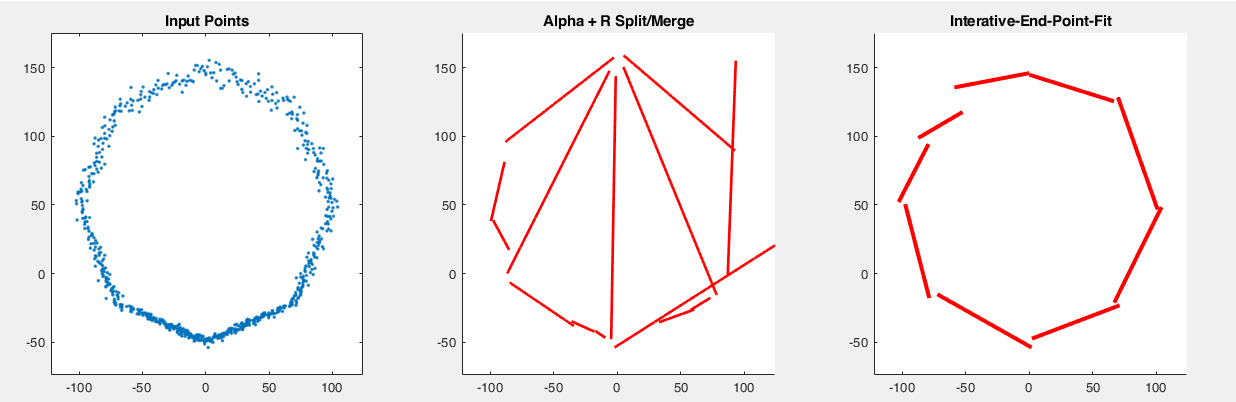
\includegraphics[width=0.8\textwidth]{p1ex1}
		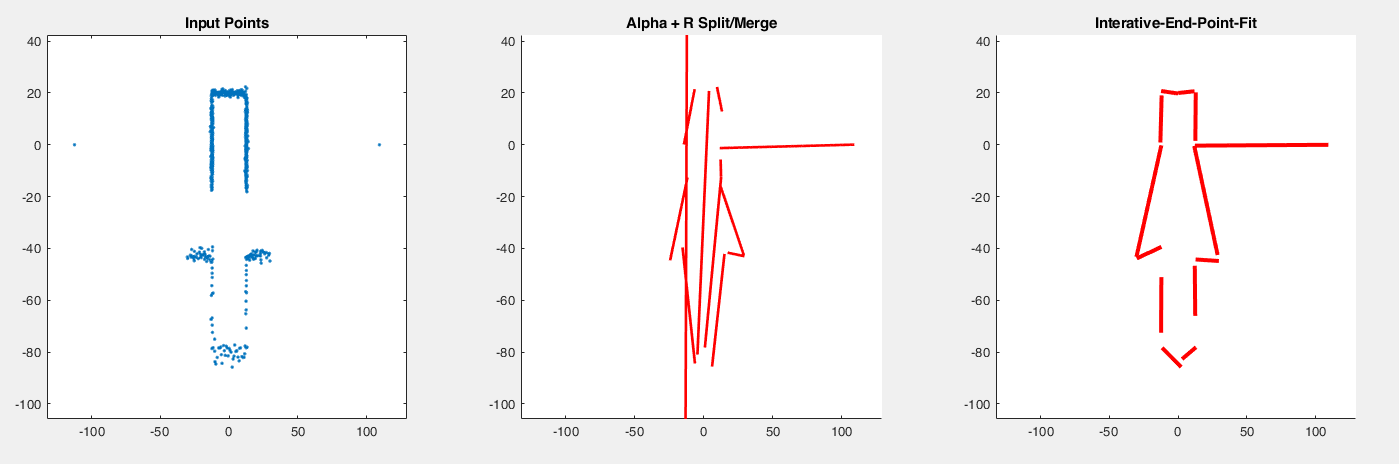
\includegraphics[width=0.8\textwidth]{p1ex2}
		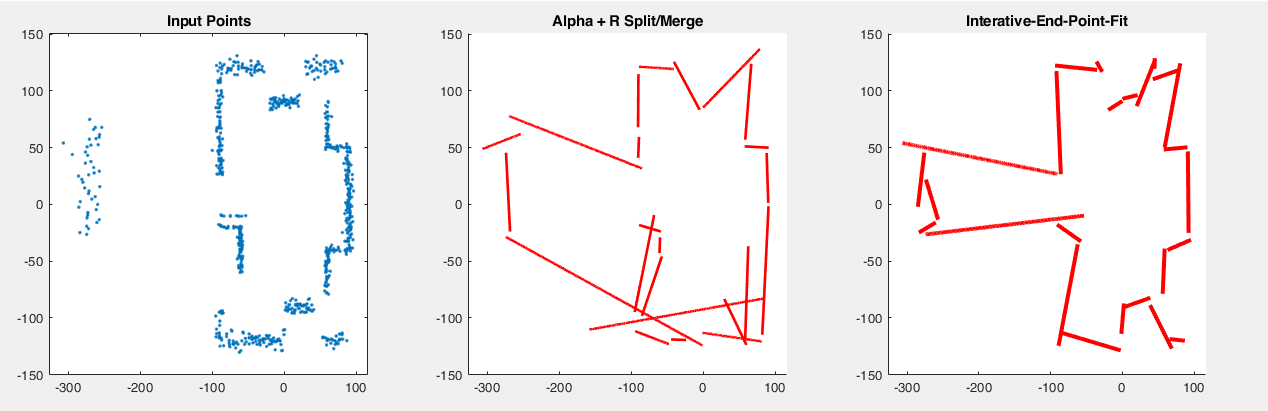
\includegraphics[width=0.8\textwidth]{p1ex3}
	\end{center}
	
	\section{Trilateration}
	
	To find our position, first I needed to find the intersections of every combination of two circles. To do this, I attempted to use the methodology discussed in class, where we use the equations of the circles to find their common points. I ran into some issues given the amount of square roots within the calculations, where in each I had to handle the negative and positive result. This was causing me some issues so I decided to go with a more trigonometric approach to the problem. Below is a diagram showing the line segments that I used to calculate the points of intersection for each circle combination.
	
	\begin{center}
	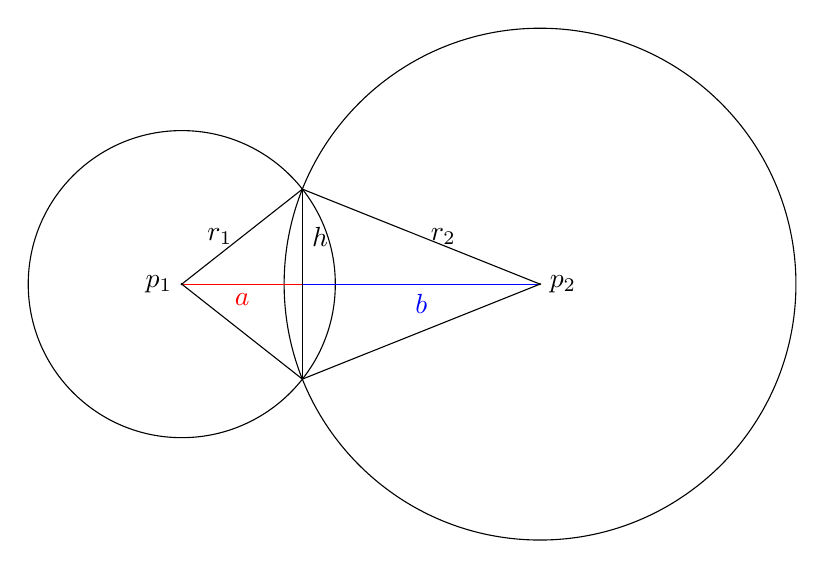
\begin{tikzpicture}[scale=0.65]
	
	\draw (1,0) circle (0.01cm) node[left] {$p_1$};
	\draw (1,0) circle (3cm);
	\draw (8,0) circle (0.01cm) node[right] {$p_2$};
	\draw (8,0) circle (5cm);
	\draw[red] (1,0) -- node[below] {$a$} ++ (2.3571, 0);
	\draw[blue] (3.3571, 0) -- node[below] {$b$} ++ (4.6429, 0);
	\draw (3.3571, 0) -- node[right] {$h$} ++ (0, 1.8558);
	\draw (3.3571, 0) -- ++ (0, -1.8558);
	\draw (1, 0) -- node[left] {$r_1$} ++ (2.3571, 1.8558);
	\draw (1, 0) -- ++ (2.3571, -1.8558);
	\draw (8, 0) -- node[right] {$r_2$} ++ (-4.6429, 1.8558);
	\draw (8, 0) -- ++ (-4.6429, -1.8558);
	
	\end{tikzpicture}
	\end{center}
	
	Firstly, I had to check that the circles are close enough to overlap. This is an easy calculation, as you simply check if $ d > r_1 + r_2$. If it turns out that the circles are too far apart, I used the point between the circles (proportional to the radius of each circle) as the only 'intersection point'.
	
	If the circles do overlap, we can find the point between the two intersection points. Using the Pythagorean Theorem, we can write the equations:
	
	\[
		a^2 + h^2 = r_1^2 \text{ and } b^2 + h^2 = r_2^2
	\]
	
	\noindent From these we can solve for a ($d = a + b$), and get
	
	\[
		a = \cfrac{r_1^2 - r_1^2 + d^2}{2 d}
	\]
	
	\noindent With $a$, we can solve the right triangle with sides $a$, $h$, and $r_1$ to get the intersection points.
	
	With these two intersection points, I calculate their distance to the third circle. I compare these distances to the distance from the third beacon to the goal. The intersection point with a distance closer to distance of the third beacon. After looping through all three combinations of circles, I'm left with 3 'good' intersection points. I use the centroid of these 3 points as my return value.
	
	\section{Triangulation}

	To estimate our position in problem three, I found the intersection point of each line with each of the other lines. I placed my beacons in the corners of the field. This caused some errors when I used the intersection point with beacons opposite each other on the grid. Because of this, I only used the two intersection points of the next beacon around the board. Using this method, I obtained four 'good' intersection points and my estimate was the centroid of these points. Below is an example output of this method. The black points are the good intersection points, the red dot is the estimated position and the red x is the actual position.
	
	\begin{center}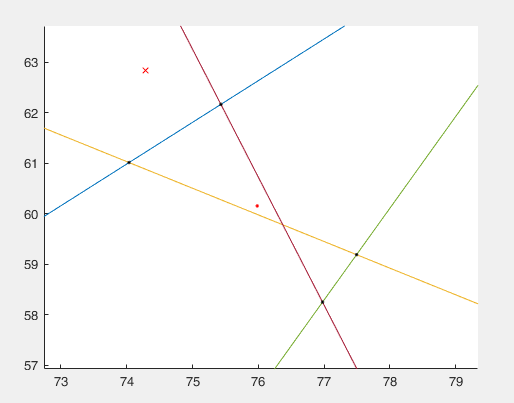
\includegraphics[width=0.8\textwidth]{p3ex}\end{center}
	
	\pagebreak
	
	\section{Code}
	
	\lstinputlisting[title=Problem 1: exam3\_q1.m]{../estimate/exam3_q1.m}
	
	\pagebreak
	
	\lstinputlisting[title=Problem 2: exam3\_q2.m]{../beacon_dist/exam3_q2.m}
	
	\pagebreak
	
	\lstinputlisting[title=Problem 3: exam3\_q3.m]{../beacon_angle/exam3_q3.m}

\end{document}